\documentclass[landscape, 8pt]{extarticle}
% \usepackage{showframe}

\usepackage[dvipsnames]{xcolor}
% custom colour definitions
\colorlet{colour1}{Red}
\colorlet{colour2}{Green}
\colorlet{colour3}{Cerulean}

\usepackage{geometry}
% margins
\geometry{
    a4paper, 
    margin=0.17in
}

\usepackage{graphicx} % Required for inserting images
\usepackage{amsmath}
\usepackage{amsfonts}
\usepackage{amssymb}
\usepackage{preamble}
\usepackage{multicol}
\usepackage{lipsum}
\usepackage{float}
\usepackage[nodisplayskipstretch]{setspace}


% tikz and theorem boxes
\usepackage[framemethod=TikZ]{mdframed}
\usepackage{../thmboxes_white}
% \usepackage{../thmboxes_col}


% Custom Definitions of operators
\DeclareMathOperator{\Ima}{im}
\DeclareMathOperator{\Fix}{Fix}
\DeclareMathOperator{\Orb}{Orb}
\DeclareMathOperator{\Stab}{Stab}
\DeclareMathOperator{\send}{send}
\DeclareMathOperator{\dom}{dom}
\DeclareMathOperator{\sech}{sech}
\DeclareMathOperator{\csch}{csch}

\begin{document}

% vertical gap between full length math mode equations
\setlength{\abovedisplayskip}{3.5pt}
\setlength{\belowdisplayskip}{3.5pt}
\setlength{\abovedisplayshortskip}{3.5pt}
\setlength{\belowdisplayshortskip}{3.5pt}

\begin{multicols}{3}
\raggedcolumns % don't force squeeze width of columns
\section{\huge Geometry Sheet - WIP}
\vspace{-5pt}

\subsection*{Definitions and stuff}

\begin{dfn}[Standard Hyperbolic Derivatives]{def:hbol_derivs}{A}
    \begin{align*}
        y = \sinh(x) & \implies \quad y' = \cosh(x) \\
        y = \cosh(x) & \implies \quad y' = \sinh(x) \\
        y = \tanh(x) & \implies \quad y' = \sech^{2}(x) \\
        y = \csch(x) & \implies \quad y' = -\csch(x)\coth(x) \\
        y = \sech(x) & \implies \quad y' = -\sech(x)\tanh(x) \\
        y = \coth(x) & \implies \quad y' = -\csch^{2}(x)
    \end{align*}
\end{dfn}
\vspace{-5pt}

\begin{dfn}[Standard Hyperbolic Identities]{def:hbol_identities}{B}
    \begin{align*}
        \tanh(x) = \frac{\sinh(X)}{\cosh(X)} & \qquad \coth(x) = \frac{\cosh(x)}{\sinh(x)} \\
        \sech(x) = \frac{1}{\cosh(x)} & \qquad \csch(x) = \frac{1}{\sinh(x)}
    \end{align*}
\end{dfn}
\vspace{-5pt}

\begin{dfn}[Cross Product]{def:cross_product}{C}
    \[
    \begin{pmatrix}
        a_{1} \\
        a_{2} \\
        a_{3}
    \end{pmatrix} \times \begin{pmatrix}
        b_{1} \\
        b_{2} \\
        b_{3}
    \end{pmatrix} = \begin{pmatrix}
        (a_{2} \cdot b_{3}) - (a_{3} \cdot b_{2}) \\
        (a_{3} \cdot b_{1}) - (a_{1} \cdot b_{3}) \\
        (a_{1} \cdot b_{2}) - (a_{2} \cdot b_{1}) \\
    \end{pmatrix}
    \]
\end{dfn}
\vspace{-5pt}

\begin{dfn}[Taylor Series Expansion]{def:taylor}{D}
\[f(x) = f(a) + f'(a)(x-a) + \frac{f''(a)}{2!}(x-a)^{2} + \frac{f^{(3)}(a)}{3!}(x-a)^{3}+ \cdots\]
Bonus: quick unit form parameterised derivations of \(x\)
\renewcommand\labelitemi{\tiny$\bullet$}
\begin{itemize}
    \setlength\itemsep{0em}
    \item \(x'(s) = T(s)\) \\
    \item \(x''(s) = T'(s) = \kappa(s)N(s)\) \\
    \item \(x'''(s) = \frac{d\kappa}{ds}(s)N(s) - \kappa^{2}(s)T(s) + \kappa(s)\tau(s)B(s)\)
\end{itemize}
\end{dfn}



\begin{dfn}[Gauss Curvature on a Graph]{thm:thm_example}{E}
Random equation that was in 2022 PP sols, can't find it anywhere in the book. Presumably only works on a graph, i.e.
\[x : (u,v) \mapsto \begin{pmatrix}
    u \\
    v \\
    f(u,v)
\end{pmatrix}\]
Equation is as follows
\[K = \frac{f_{uu} f_{vv} - f_{uv}^{2}}{(1 + f^{2}_{u} + f^{2}_{v})^{2}}\]
\end{dfn}
\vspace{-5pt}

\begin{dfn}[Closed vs Exact Forms]{def:closed-exact}{F}
A form \(\alpha\in \Omega^{K}(D)\) is said to be \textbf{closed} if \(d\alpha = 0\) and is said to be \textbf{exact} if \(\alpha = d\beta\) for some \(\beta\in \Omega^{k-1}(D)\)\newline
Every exact form is closed, since \(d^{2} = 0\). The converse is not neccesarily true\newline
If \(\alpha\) is exact, and \(\beta\) is closed, then \(\alpha \wedge \beta\) is also exact

\end{dfn}

\begin{dfn}[Hyperbolic plane representations]{def: poincare}{G}
    Poincare Upper half plane model
    \begin{figure}[H]
        \centering
        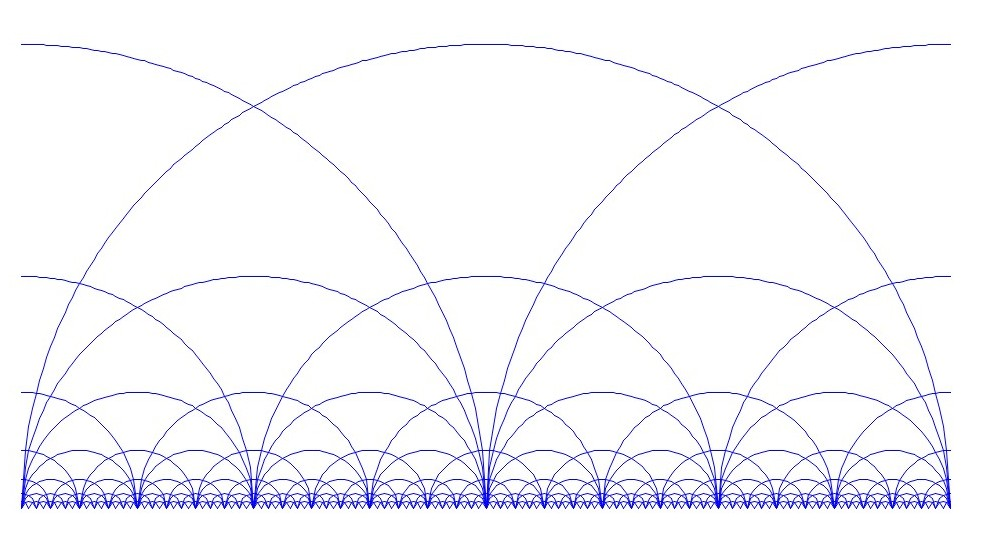
\includegraphics[width=\linewidth]{images/halfplane1.jpg}
    \end{figure}
    
    Poincare Hyperbolic disk model
    \begin{figure}[H]
        \centering
        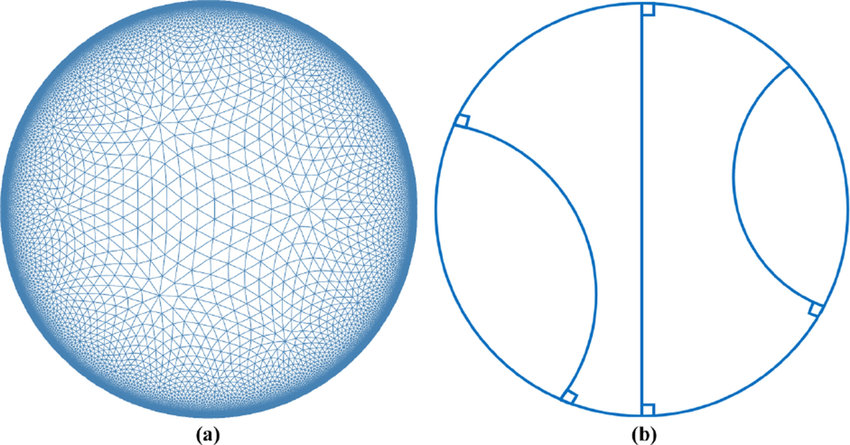
\includegraphics[width=\linewidth]{images/diskmodel.jpg}
    \end{figure}
\end{dfn}

\begin{dfn}[Standard Orientation]{def:standard-orientation}{H}
The \textbf{standard orientation} (which we always assume) is defined by
\[dx^{1} \wedge dx^{2}\wedge \cdots \wedge dx^{n}\]
Coordinates \((y^{1},\dots,y^{n})(\text{an ordered set})\) are said to be \textbf{oriented} on \(D\) iff \(dy^{1}\wedge \cdots \wedge dy^{n}\) is a positive multiple of \(dx^{1}\wedge \cdots \wedge dx^{n}\) for all \(x\in D \subseteq \mathbb{R}^{n}\)
\end{dfn}

\begin{dfn}[Unit Frame Vector Diagram]{def:serrat-frame-diagram}{I}
\begin{figure}[H]
    \centering
    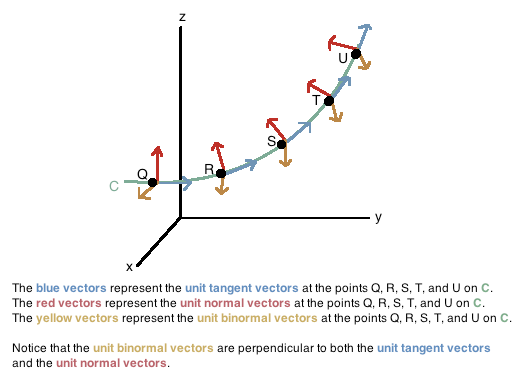
\includegraphics[width=\linewidth]{images/normal tangent.png}
\end{figure}
\end{dfn}

\begin{thm}[nah i'd win]{thm:idwin}{nah i'd win}
    \begin{figure}[H]
        \centering
        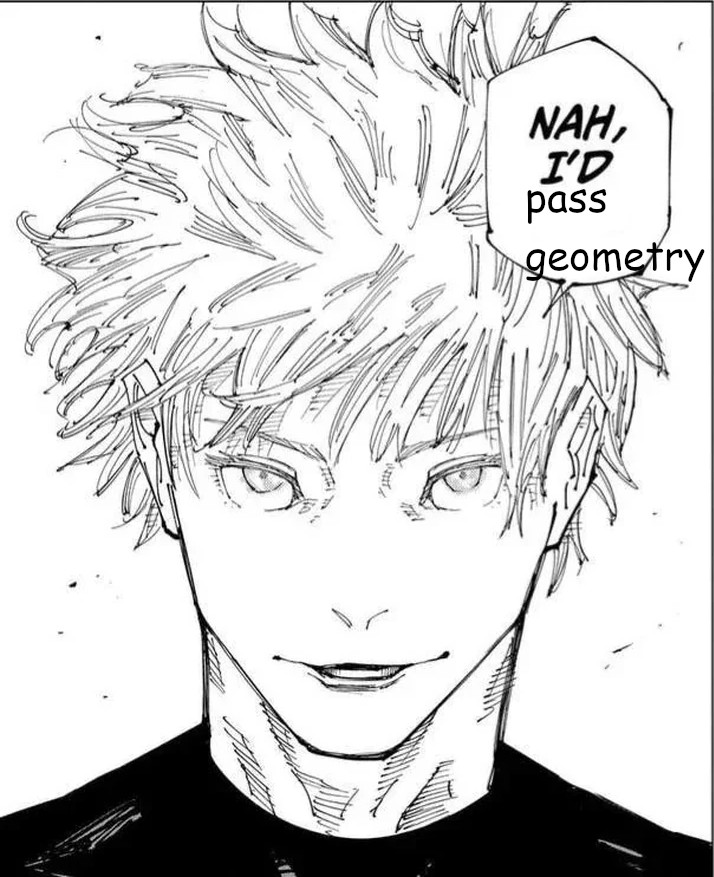
\includegraphics[width=\linewidth]{images/nah_id_win.jpg}
    \end{figure}
\end{thm}

\newpage 

\subsection*{Examples}

\begin{xmp}[Wedge Product Exmaple]{def:wedge}{1}
Find the wedge product of 
\[(x^{1}dx^{2} - dx^{3}) \wedge ((x^{1})^{2}dx^{1}\wedge dx^{2} + x^{3}dx^{1}\wedge dx^{3})\]
\begin{align*}
   &(x^{1}dx^{2} - dx^{3}) \wedge ((x^{1})^{2}dx^{1}\wedge dx^{2} + x^{3}dx^{1}\wedge dx^{3}) \\
    &= \textcolor{red}{0} + x^{1}x^{3}dx^{2}\wedge dx^{1}\wedge dx^{3} - (x^{1})^{2}dx^{3}\wedge dx^{1}\wedge dx^{2} - \textcolor{red}{0} \\
    &= x^{1}x^{3}dx^{2}\wedge dx^{1}\wedge dx^{3} - (x^{1})^{2}dx^{3}\wedge dx^{1}\wedge dx^{2} \\
    &= \textcolor{blue}{-}x^{1}x^{3}dx^{\textcolor{blue}{1}}\wedge dx^{\textcolor{blue}{2}}\wedge dx^{3} \textcolor{blue}{+} (x^{1})^{2}dx^{\textcolor{blue}{1}}\wedge dx^{\textcolor{blue}{3}}\wedge dx^{2} \\
    &= -x^{1}x^{3}dx^{1}\wedge dx^{2}\wedge dx^{3} \textcolor{blue}{-} (x^{1})^{2}dx^{1}\wedge dx^{\textcolor{blue}{2}}\wedge dx^{\textcolor{blue}{3}} \\
    &= -x^{1}(x^{3} + x^{1} )dx^{1}\wedge dx^{2}\wedge dx^{3}
\end{align*}
\end{xmp}


\begin{xmp}[Exterior Derivative Example]{def:ext-derivative}{2}
Find the Exterior Derivative of the 1-form \(\alpha = x^{1}x^{2}dx^{1} + x^{3}dx^{2} - dx^{3}\). (This should turn from a 1-form to a 2-form, i.e. \(\Omega^{1}(D)\to \Omega^{2}(D)\))
\begin{align*}
    \alpha &= d(x^{1}x^{2}dx^{1} + x^{3}dx^{2} - dx^{3}) \\ 
    &= d(x^{1}x^{2})\wedge dx^{1} + dx^{3}\wedge dx^{2} + \textcolor{red}{d(-1)\wedge dx^{3}} \\
    &= (x^{2}dx^{1} + x^{1}dx^{2}) \wedge dx^{1} - dx^{2}\wedge dx^{3} \\
    &= \textcolor{red}{x^{2}dx^{1}\wedge dx^{1}}-x^{1}dx^{1}\wedge dx^{2} - dx^{2} \wedge dx^{3} \\
    &= -x^{1}dx^{1}\wedge dx^{2} - dx^{2} \wedge dx^{3} 
\end{align*}

\end{xmp}

\begin{xmp}[Pullback Example]{def:pullback}{3}
Let \(f:\mathbb{R}^{2} \to \mathbb{R}^{2}\) be given by
\[f(u^{1}, u^{2}) = ((u^{1})^{2}, (u^{2})^{2}, u^{1}u^{2}))\]
where we use the Cartesian coordinates \((u^{1}, u^{2})\) on \(\mathbb{R}^{2}\) and \((x^{1}, x^{2}, x^{3})\) on \(\mathbb{R}^{3}\). Calculate the pullback \(f^{*}\rho\) for the form
\[\rho = x^{1}dx^{2}\wedge dx^{3}\]
\begin{align*}
    f^*\rho &= (u^{1})^{2}d((u^{2})^{2}) \wedge d(u^{1}u^{2}) \\
    &= (u^{1})^{2} 2u^{2}du^{2} \wedge (u^{2} du^{1} + u^{1}du^{2}) \\
    &= -2(u^{1}u^{2})^{2}du^{1} \wedge du^{2}
\end{align*}

\end{xmp}



\begin{xmp}[Theorema Egregium]{def:theorema}{4}
    Example - Finding Gauss Curvature on a sphere defined with the equation
    \[x:(\alpha, \phi)\mapsto \begin{pmatrix}
        a\sin\alpha \cos\phi \\
        a\sin\alpha \sin\phi \\
        a\cos\alpha
    \end{pmatrix}\]
    with the first fundamental form
    \[\mathrm{I} = a^{2}d\alpha^{2} + a^{2}\sin^{2}\alpha d\phi^{2}\]
    Pick \(\theta^{1}\) and \(\theta^{2}\) such that \(\mathrm{I} = (\theta^{1})^{2} + (\theta^{1})^{2}\). i.e.
    \[\theta^{1} = ad\alpha,\quad \theta^{2} = a\sin\alpha d\phi\]
    Find exterior derivatives
    \[d\theta^{1} = 0 , \quad d\theta^{2} = a\cos\alpha d\alpha\wedge d\phi\]
    Substitute into the equations \(d\theta^{1} + \omega^{1}_{2}\wedge \theta^{2} = 0\) and \(d\theta^{2} + \omega^{2}_{1}\wedge \theta^{1} = 0\)
    Substituting into the first equation, we get
    \begin{align*}
        \theta^{1} + \omega^{1}_{2}\wedge \theta^{2} = 0 &\implies 0 + \omega^{1}_{2}\wedge a\sin\alpha d\phi = 0 \\
        &\implies (a\sin\alpha) w^{1}_{2} \wedge d\phi = 0
    \end{align*}
    This implies that \(\omega^{1}_{2}\) must be proportional to \(d\phi\) only, so that the wedge product can evaluate to \(d\phi \wedge d\phi = 0\). Therefore, \(w^{1}_{2} = \psi d\phi\) for some function \(\psi\). Substituting into the second equation, we get
    \begin{align*}
        \theta^{2} + \omega^{2}_{1}\wedge \theta^{1} = 0 &\implies a\cos\alpha d\alpha\wedge d\phi + \omega^{2}_{1}\wedge ad\alpha = 0 \\
        &\implies a\cos\alpha d\alpha\wedge d\phi = -\omega^{2}_{1}\wedge ad\alpha \\
        &\implies a\cos\alpha d\alpha\wedge d\phi = a\omega^{1}_{2}\wedge d\alpha \\
        &\implies \textcolor{blue}{\cos\alpha} d\alpha\wedge \textcolor{blue}{d\phi} = \textcolor{blue}{\omega^{1}_{2}}\wedge d\alpha \\
    \end{align*}
    This can then be solved by having \(\omega^{1}_{2} = -cos\alpha d\phi\) (the minus sign coz the wedge needs flipped)
    Now we can find the Gauss Curvature with the equation
    \[d\omega^{1}_{2} = K\theta^{1}\wedge \theta^{2}\]
    by substituting values for \(\theta^{1}\) and \(\theta^{2}\), and finding the exterior derivative of \(\omega^{1}_{2}\)
    \begin{align*}
        \omega^{1}_{2} &= -\cos\alpha d\phi \\
        \implies d\omega^{1}_{2} &= \sin\alpha d\alpha\wedge d\phi
    \end{align*}
    Compare to wedge
    \begin{align*}
        \sin\alpha d\alpha\wedge d\phi &= K (ad\alpha) \wedge (a\sin\alpha d\phi) \\
        \sin\alpha d\alpha\wedge d\phi&= K a^{2}\sin\alpha d\alpha\wedge d\phi
    \end{align*}
    Therefore, \(\displaystyle K = \frac{1}{a^{2}}\)
\end{xmp}

\begin{xmp}[random q]{thm:random_q_1}{5}
    I was just doing this on latex to be neater cos the calculations were really tedious, might remove later idk

    Find the exterior derivative of
    \[\beta = \frac{x^{1}dx^{2} - x^{2}dx^{1}}{(x^{1})^{2} + (x^{2})^{2}}\]
    Let \(f\) be the function 
    \[\displaystyle f = \frac{1}{(x^{1})^{2} + (x^{2})^{2}} = ((x^{1})^{2} + (x^{2})^{2})^{-1}\]
    Then, we have 
    \begin{align*}
        df &= \displaystyle\frac{\partial f}{\partial x^{1}}dx^{1} + \frac{\partial f}{\partial x^{2}} dx^{2} \\
        &= - \frac{2x^{1}}{((x^{1})^{2} + (x^{2})^{2})^{2}}dx^{1} - \frac{2x^{2}}{((x^{1})^{2} + (x^{2})^{2})^{2}}dx^{2}
    \end{align*}
    Returning to the original equation, rewrite as follows
    \begin{align*}
        \beta &= f(x^{1}dx^{2} - x^{2}dx^{1}) \\
        &= fx^{1}dx^{2} - fx^{2}dx^{1} \\
        d\beta &= d(fx^{1}) \wedge dx^{2} - d(fx^{2}) \wedge dx^{1} \\
        &= (x_{1}df + fdx^{1}) \wedge dx^{2} - (x^{2}df + fdx^{2}) \wedge dx^{1} \\
        &= x^{1}df\wedge dx^{2} + \frac{dx^{1}\wedge dx^{2}}{(x^{1})^{2} + (x^{2})^{2}} - x^{2}df\wedge dx^{1} - \frac{dx^{2}\wedge dx^{1}}{(x^{1})^{2} + (x^{2})^{2}} \\
        &= \frac{2dx^{1}\wedge dx^{2}}{(x^{1})^{2} + (x^{2})^{2}} + x^{1}df\wedge dx^{2} - x^{2}df\wedge dx^{1} \\
        &= \frac{2dx^{1}\wedge dx^{2}}{(x^{1})^{2} + (x^{2})^{2}} + x^{1} \left(- \frac{2x^{1}}{((x^{1})^{2} + (x^{2})^{2})^{2}}\right)dx^{1} \wedge dx^{2} \\
        &+ x^{2} \left(- \frac{2x^{2}}{((x^{1})^{2} + (x^{2})^{2})^{2}}\right)dx^{2} \wedge dx^{1} \\
        &= \frac{2dx^{1}\wedge dx^{2}}{(x^{1})^{2} + (x^{2})^{2}} -  \left(\frac{2(x^{1})^{2}}{((x^{1})^{2} + (x^{2})^{2})^{2}}\right)dx^{1} \wedge dx^{2} \\
        &+ \left(\frac{2(x^{2})^{2}}{((x^{1})^{2} + (x^{2})^{2})^{2}}\right)dx^{1} \wedge dx^{2} \\
        &= \frac{2dx^{1}\wedge dx^{2}}{(x^{1})^{2} + (x^{2})^{2}} -  \frac{2((x^{1})^{2} + 2(x^{2})^{2})dx^{1} \wedge dx^{2}}{((x^{1})^{2} + (x^{2})^{2})^{2}} \\ 
    \end{align*}
    

\end{xmp}
\vspace{-5pt}

% Add a new page if a box gets cut off 


% blank filler text
% \lipsum[1-12]

\end{multicols}

\end{document}